\documentclass[margin,line]{res}

\usepackage{graphicx}
\usepackage{float}
\usepackage{tabularx}
\usepackage{hyperref}
\hypersetup{
  colorlinks   = true, %Colours links instead of ugly boxes
  urlcolor     = blue, %Colour for external hyperlinks
  linkcolor    = blue, %Colour of internal links
  citecolor   = red %Colour of citations
}

\oddsidemargin -.5in
\evensidemargin -.5in
\textwidth=6.0in
\itemsep=0in
\parsep=0in
% if using pdflatex:
\setlength{\pdfpagewidth}{\paperwidth}
\setlength{\pdfpageheight}{\paperheight} 

\newenvironment{list1}{
  \begin{list}{\ding{113}}{%
      \setlength{\itemsep}{0in}
      \setlength{\parsep}{0in} \setlength{\parskip}{0in}
      \setlength{\topsep}{0in} \setlength{\partopsep}{0in} 
      \setlength{\leftmargin}{0.17in}}}{\end{list}}
\newenvironment{list2}{
  \begin{list}{$\bullet$}{%
      \setlength{\itemsep}{0in}
      \setlength{\parsep}{0in} \setlength{\parskip}{0in}
      \setlength{\topsep}{0in} \setlength{\partopsep}{0in} 
      \setlength{\leftmargin}{0.2in}}}{\end{list}}


\begin{document}

\name{Daobilige Su \vspace*{.1in}}

\begin{resume}



%%%%%%%%%%%%
\section{\sc Contact Information}
\vspace{.05in}
\begin{tabularx}{\textwidth}{X r}
Australian Centre for Field Robotics (ACFR),      &  +61(0)-410-891-777 \\            
The Rose Street Building, University of Sydney,   & daobilige.su@gmail.com \\
Camperdown, NSW 2006, Australia   & \\%{\it E-mail:}  paciorek@stat.cmu.edu\\       
%  & \\%{\it WWW:} www.stat.cmu.edu/\verb+~+paciorek \\     
\end{tabularx}



%%%%%%%%%%%%
\section{\sc Research Interests}
Field Robotics for Precision Agriculture, SLAM, Deep Learning for Robot Vision, Autonomous Navigation and Robot Audition


%%%%%%%%%%%%
\section{\sc Current Occupation}
\begin{tabularx}{\textwidth}{X r}
%\href{http://www.uts.edu.au}{{\bf University of Sydney}}, Sydney, Australia  
{\bf PostDoc Research Associate}, &Mar, 2017 - present\\
\end{tabularx}
%{\em Department of Statistics} 
\vspace*{-.1in}
\begin{list1}
\item[] \href{https://sydney.edu.au/engineering/our-research/robotics-and-intelligent-systems/australian-centre-for-field-robotics.html}{Australian Centre for Filed Robotics (ACFR)}, \\%\\ {\it Expected:} Jan. 2017
\href{https://sydney.edu.au/}{{The University of Sydney}}, Sydney, Australia
\begin{list2}
\vspace*{.05in}
\item Research Topic:  ``Intelligent Perception Systems for Agriculture and the Environment'' 
%\item Dissertation Topic:  ``Hierarchical Models for Multiple Ratings
%  in Performance-Based\\ \hspace*{1.23in} Student Assessments.'' 
\item Supervisor: \href{http://sydney.edu.au/engineering/people/salah.sukkarieh.php}{Prof. Salah Sukkarieh}%, \href{http://sydney.edu.au/engineering/people/james.underwood.php}{Dr. James Underwood}
\item \textbf{Robots}: \href{https://confluence.acfr.usyd.edu.au/display/AGPub/Our+Robots}{\textbf{Ladybird, RIPPA and Digital Farmhand}}(\href{https://sydney.edu.au/engineering/our-research/robotics-and-intelligent-systems/australian-centre-for-field-robotics/agriculture-and-the-environment.html}{alternative link})
\end{list2}
\end{list1}

\begin{figure}[H]
  \centering
  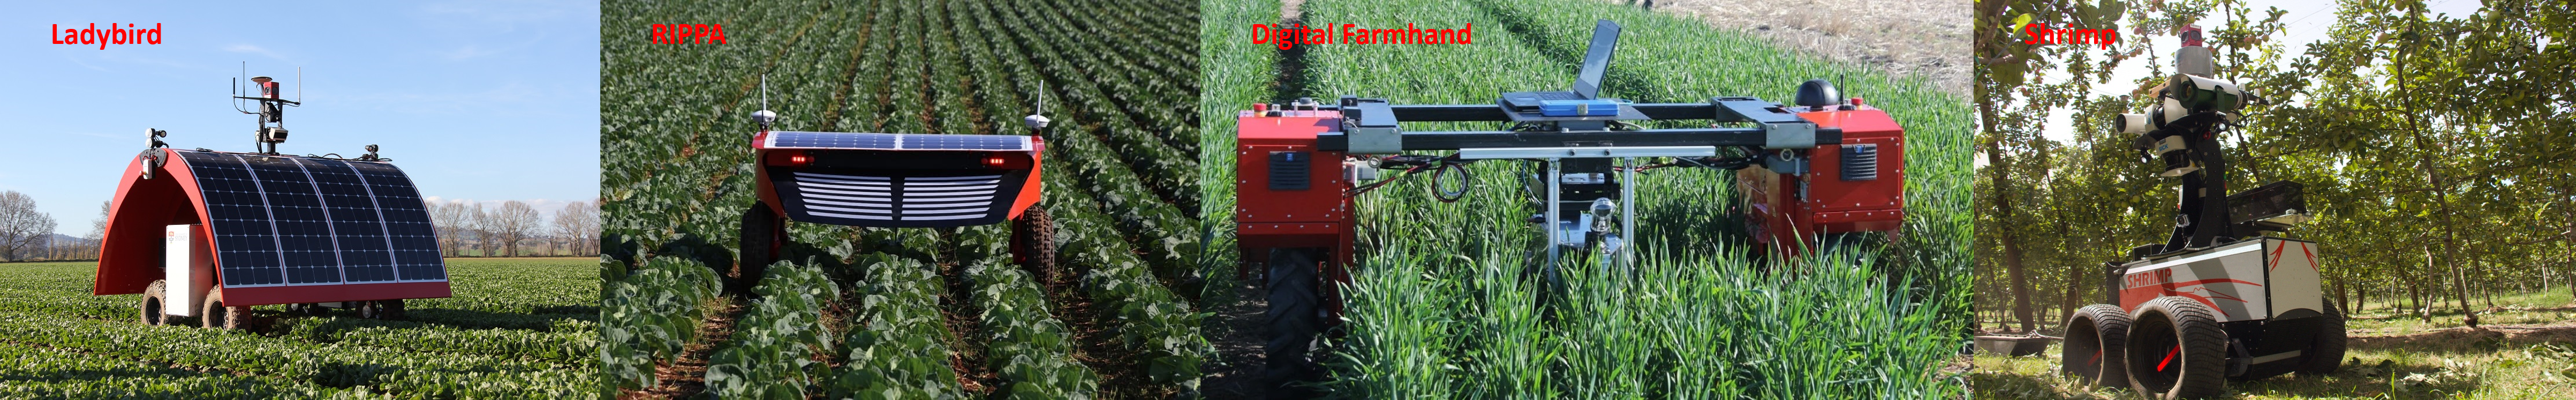
\includegraphics[width=0.99\columnwidth]{./figs/ladybird_rippa_digitalfarmhand_shrimp.png}
  %\caption{The architecture of non-bottleneck-1D block.}
  \label{fig:ladybird_rippa_digitalfarmhand_shrimp}
\end{figure}
%%%%%%%%%%%%


%%%%%%%%%%%%
\section{\sc Education}
\begin{tabularx}{\textwidth}{X r}
\href{http://www.uts.edu.au}{{\bf University of Technology Sydney (UTS)}}, Sydney, Australia  &Mar, 2013 - Mar, 2017\\
\end{tabularx}
%{\em Department of Statistics} 
\vspace*{-.1in}
\begin{list1}
\item[] Ph.D. Candidate on Robotics at \href{http://www.cas.uts.edu.au}{Centre for Autonomous System}%\\ {\it Expected:} Jan. 2017
\begin{list2}
\vspace*{.05in}
\item Dissertation Topic:  ``Robotic Sound Source Mapping using Microphone Arrays'' 
%\item Dissertation Topic:  ``Hierarchical Models for Multiple Ratings
%  in Performance-Based\\ \hspace*{1.23in} Student Assessments.'' 
\item Supervisor: \href{http://www.uts.edu.au/staff/jaime.vallsmiro}{A/Prof. Jaime Valls Miro}
\item Co-supervisor:  \href{http://www.uts.edu.au/staff/teresa.vidalcalleja}{Dr. Teresa Vidal Calleja}
\end{list2}
\end{list1}

\begin{tabularx}{\textwidth}{X r}
\href{http://emaro.irccyn.ec-nantes.fr/}{{\bf EMARO} (European Master on Advanced RObotics)} &Oct, 2010 - Oct, 2012\\
\end{tabularx}
%{\em Department of Mathematics and Statistics} 
\vspace*{-.1in}
\begin{list1}
\item[] University of Genova, Italy (Oct, 2011 - Oct, 2012)
\begin{list2}
\vspace*{.05in}
\item Master of Automation, GPA: 92/100
\end{list2}
\begin{list2}
\vspace*{.05in}
\item Master thesis at Keio University, Japan (Apr, 2012 - Sep, 2012)\\
Thesis topic: Designing Real-Time Robot Audition System\\
Thesis supervisor: Prof. Nozumo Hamada
\end{list2}
\end{list1}
\begin{list1}
\item[] Warsaw University of Technology, Poland (Oct, 2010 - Jul, 2011)
\begin{list2}
\vspace*{.05in}
\item Master of Automation and Robotics, GPA: 81.5/100
\end{list2}
\end{list1}

\begin{tabularx}{\textwidth}{X r}
\href{http://www.zju.edu.cn/english/}{{\bf Zhejiang University}}, Hangzhou, China   &Sep, 2006 - Jul, 2010\\
\end{tabularx}
%{\em Department of Mathematics and Statistics} 
\vspace*{-.1in}
\begin{list1}
\item[] Bachelor of Mechatronic Engineering, GPA: 3.63/4.0 (last 2 years:3.76/4.0)
\end{list1}

%%%%%%%%%%%%
\section{\sc Academic Experience}

\begin{tabularx}{\textwidth}{X r}
{\bf Summer School} & Feb, 2015\\
\end{tabularx}
\begin{itemize}
\item[] \href{http://rp-www.cs.usyd.edu.au/~mlss/}{2015 Machine Learning Summer School}, University of Sydney, Australia

\vspace*{-2.5mm}
\item[] Bayesian Inference and MCMC, Structured Prediction, Bayesian Nonparametrics, Natural Language Processing, Deep Learning, etc.
\end{itemize}

\begin{tabularx}{\textwidth}{X r}
{\bf Summer School} & Jul, 2011\\
\end{tabularx}
\begin{itemize}
\item[] \href{http://www.asl.ethz.ch}{ASL (Autonomous Systems Lab)}, ETH Zurich, Switzerland

\vspace*{-2.5mm}
\item[] Design, Perception, and Control for Autonomous Micro Aerial Vehicles
\end{itemize}

%%%%%%%%%%%%
\section{\sc Work Experience}

\begin{tabularx}{\textwidth}{X r}
{\bf Internship} & May, 2015 - Sep, 2015\\
\end{tabularx}
\begin{itemize}
\item[] \href{http://www.jp.honda-ri.com/english}{Honda Research Institute, Japan (HRI-JP)}

\vspace*{-2.5mm}
\item[] Supervisors: Dr. Keisuke Nakamura and Prof. Kazuhiro Nakadai
\end{itemize}

\begin{tabularx}{\textwidth}{X r}
{\bf Internship} & Feb, 2010 - Jun, 2010\\
\end{tabularx}
\begin{itemize}
\item[] Bosch Power Tools (China) Co., Ltd.

\vspace*{-2.5mm}
\item[] Manufacturing Manager Assistant
\end{itemize}

%%%%%%%%%%%%
\section{\sc Selected Projects} 

\begin{itemize}
\item {\bf Intelligent Perception for Robotic Non-Chemical Weeding}\\
Sept, 2018 - now, at ACFR, The University of Sydney.\\
Development of a deep learning based method for real-time semantic segmentation of weed against crop using TensorFlow, C++ and ROS. \\
(\textbf{confidential industry project})\\
\begin{figure}[H]
  \centering
  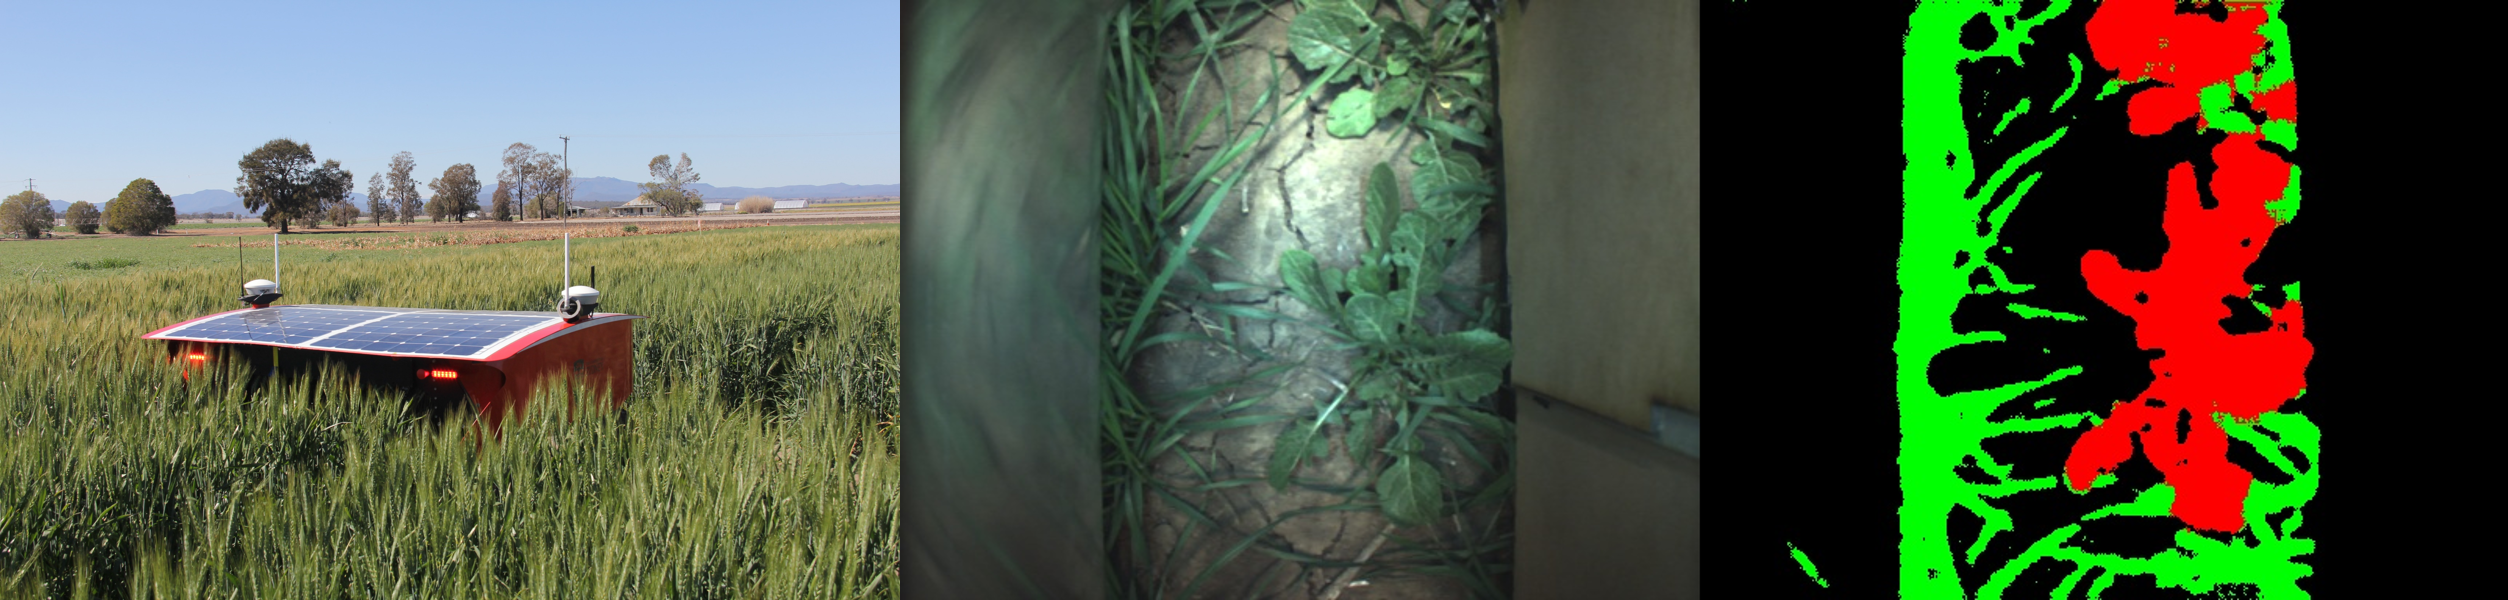
\includegraphics[width=0.9\columnwidth]{./figs/clyde_seg.png}
\end{figure}

\item {\bf Intelligent Perception for Robotic Precision Spray of Vegetable Crops }\\
Sept, 2017 - Sept, 2018, at ACFR, The University of Sydney.\\
Development of a deep learning based method to detect and track vegetable crops and leaf segmentation and localization for precision spray using TensorFlow.\\
The method allow an agricultural robot to accurately spray individual leaves of crops. \\
(\textbf{confidential industry project})\\
\begin{figure}[H]
  \centering
  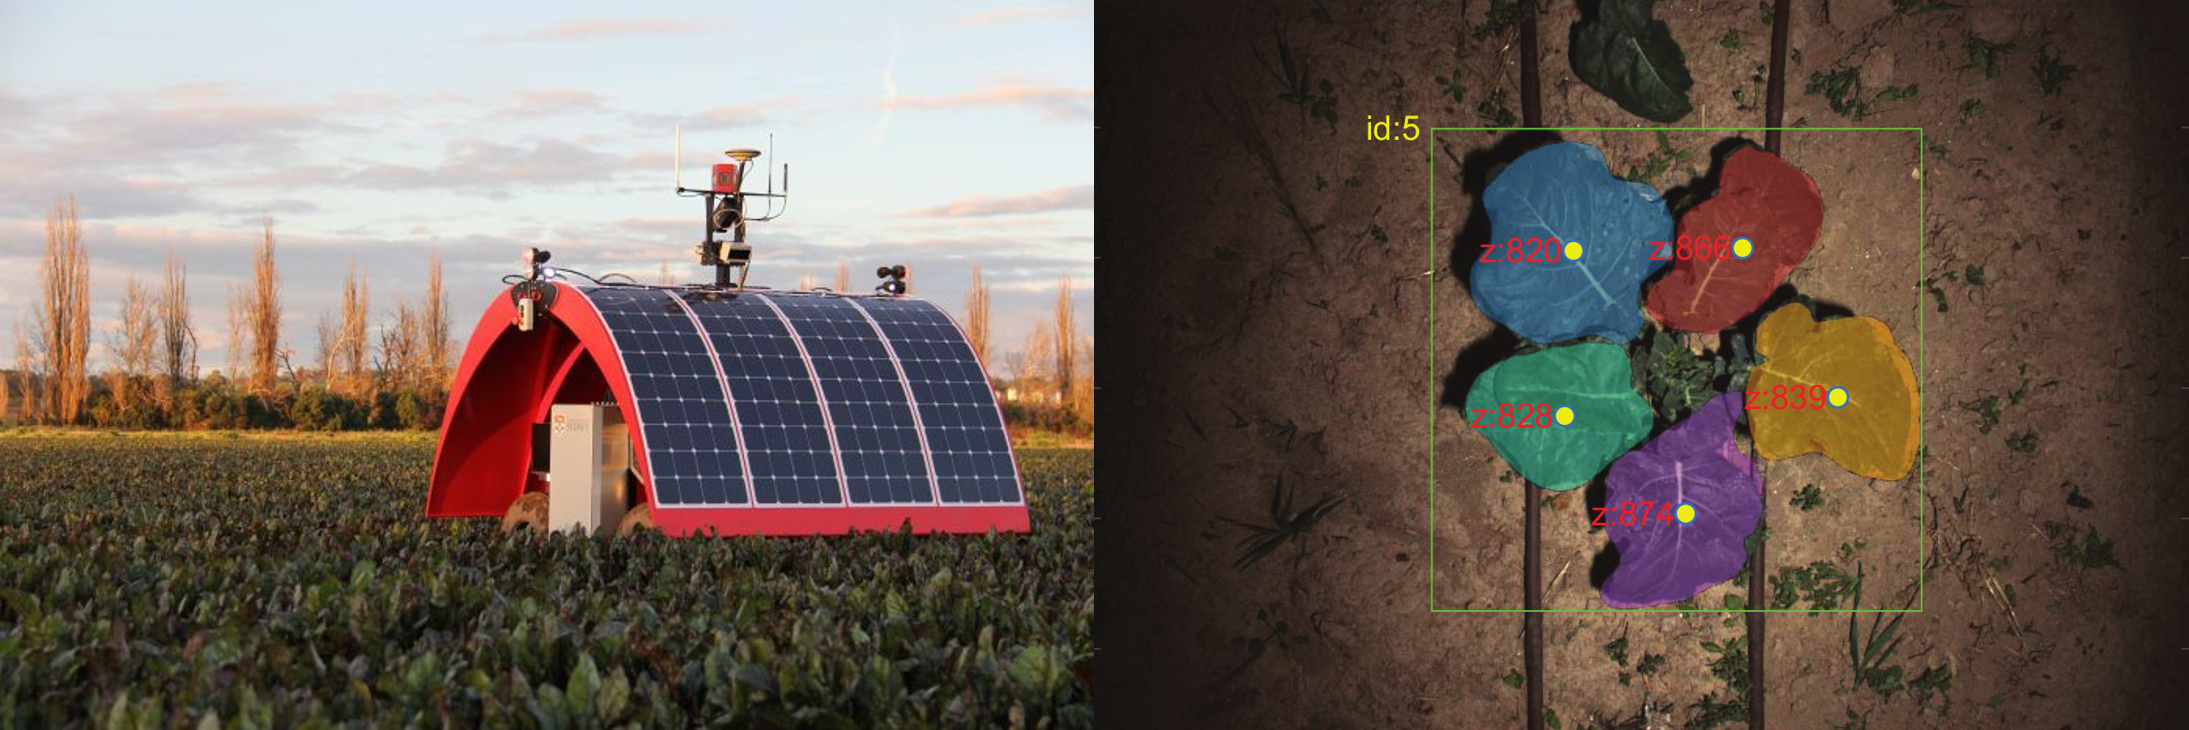
\includegraphics[width=0.62\columnwidth]{./figs/ladybird_leaf_seg.png}
\end{figure}

\item {\bf 3D Laser Scan based SLAM in Agricultural Tree Crops }\\
Mar, 2017 - Sept, 2017, at ACFR, The University of Sydney.\\
Development of a 3D Laser pointcloud based SLAM algorithm for agricultural robots in tree crops environment using Velodyne scanner.\\
(\textbf{confidential industry project})\\
\begin{figure}[H]
  \centering
  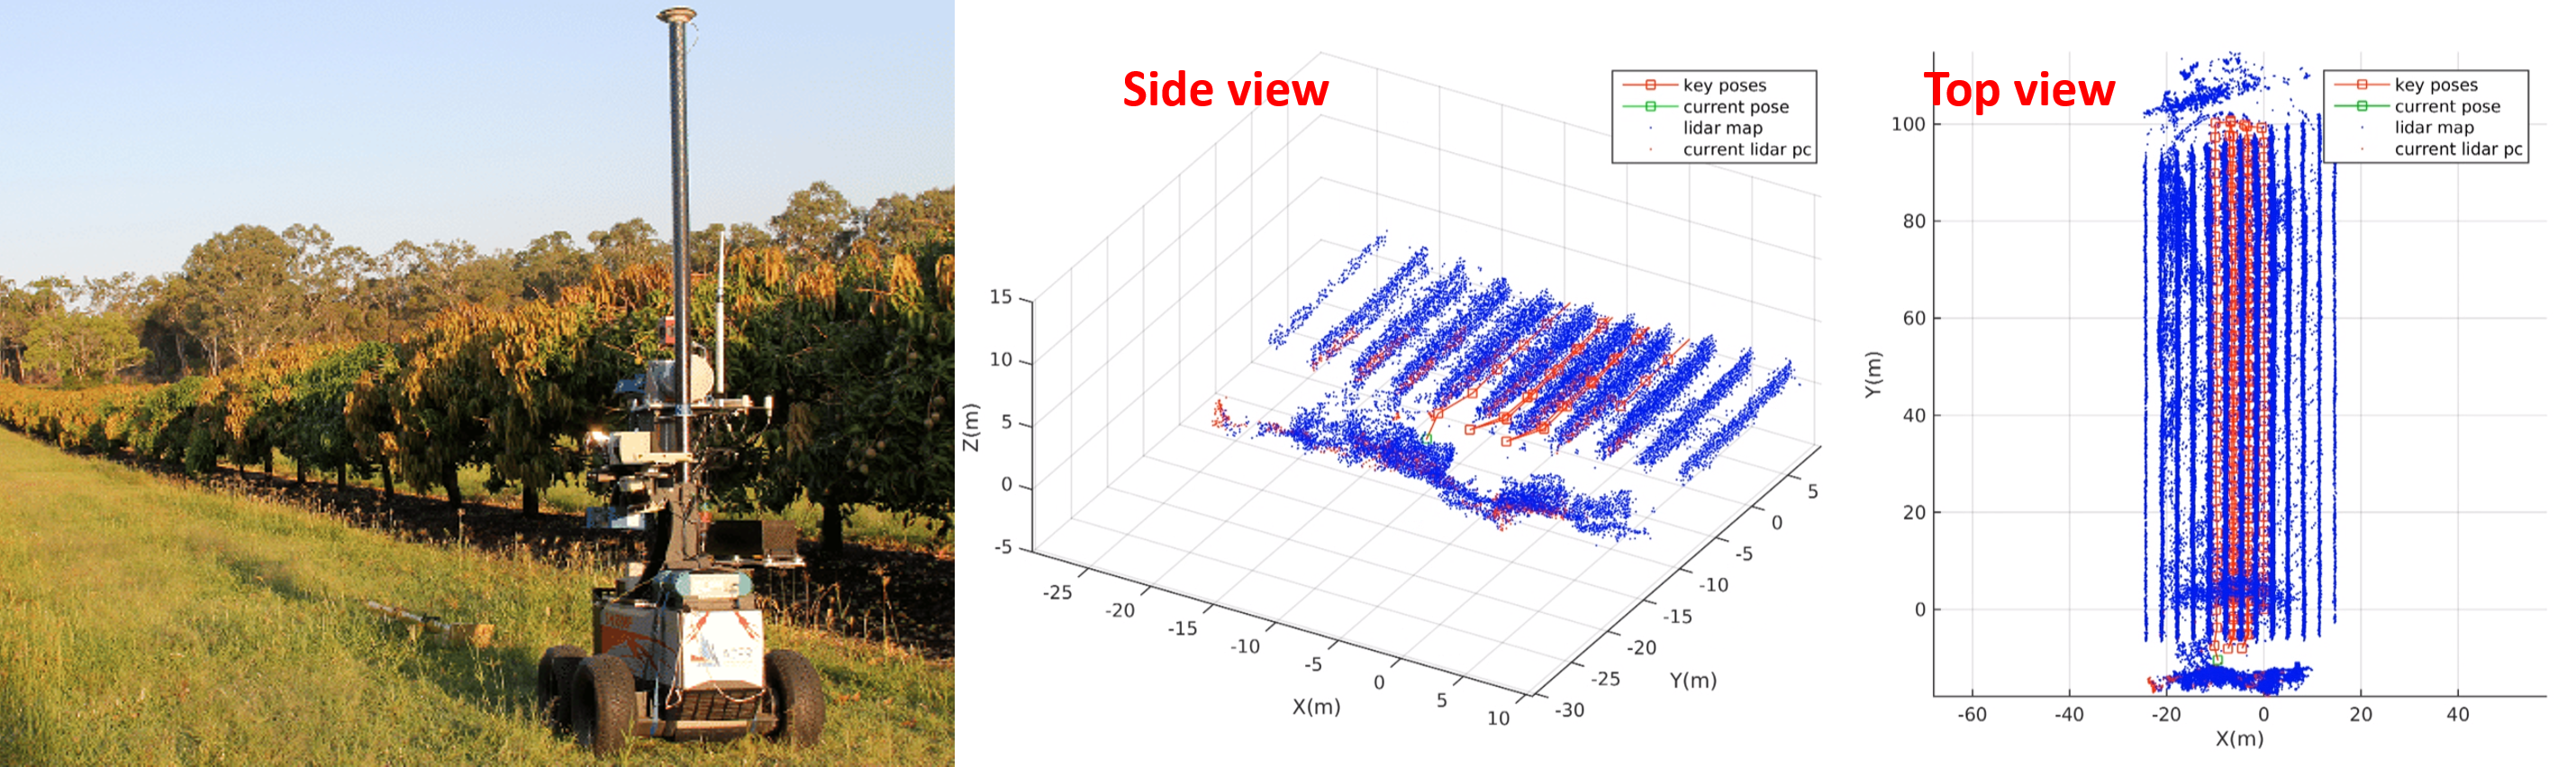
\includegraphics[width=0.9\columnwidth]{./figs/shrimp_lidar_loc.png}
\end{figure}


\item {\bf Development of an Invariant-EKF Visual Inertial Navigation System (VINS) Algorithm for Improving Consistency}\\
Sept, 2016 - Mar, 2017, at CAS, UTS.\\
Implementation of optimisation on manifold based visual inertial SLAM backend using Matlab (for simulation).\\
Implementation of MSCKF based visual inertial SLAM backend using Matlab (for simulation).\\
Visual features extraction, matching and visual place recognition using OpenCV and ORBSLAM frontend.\\
%Affiliated Video: \href{https://youtu.be/QyqY2eIX1wk}{https://youtu.be/QyqY2eIX1wk}.\\
\begin{figure}[H]
  \centering
  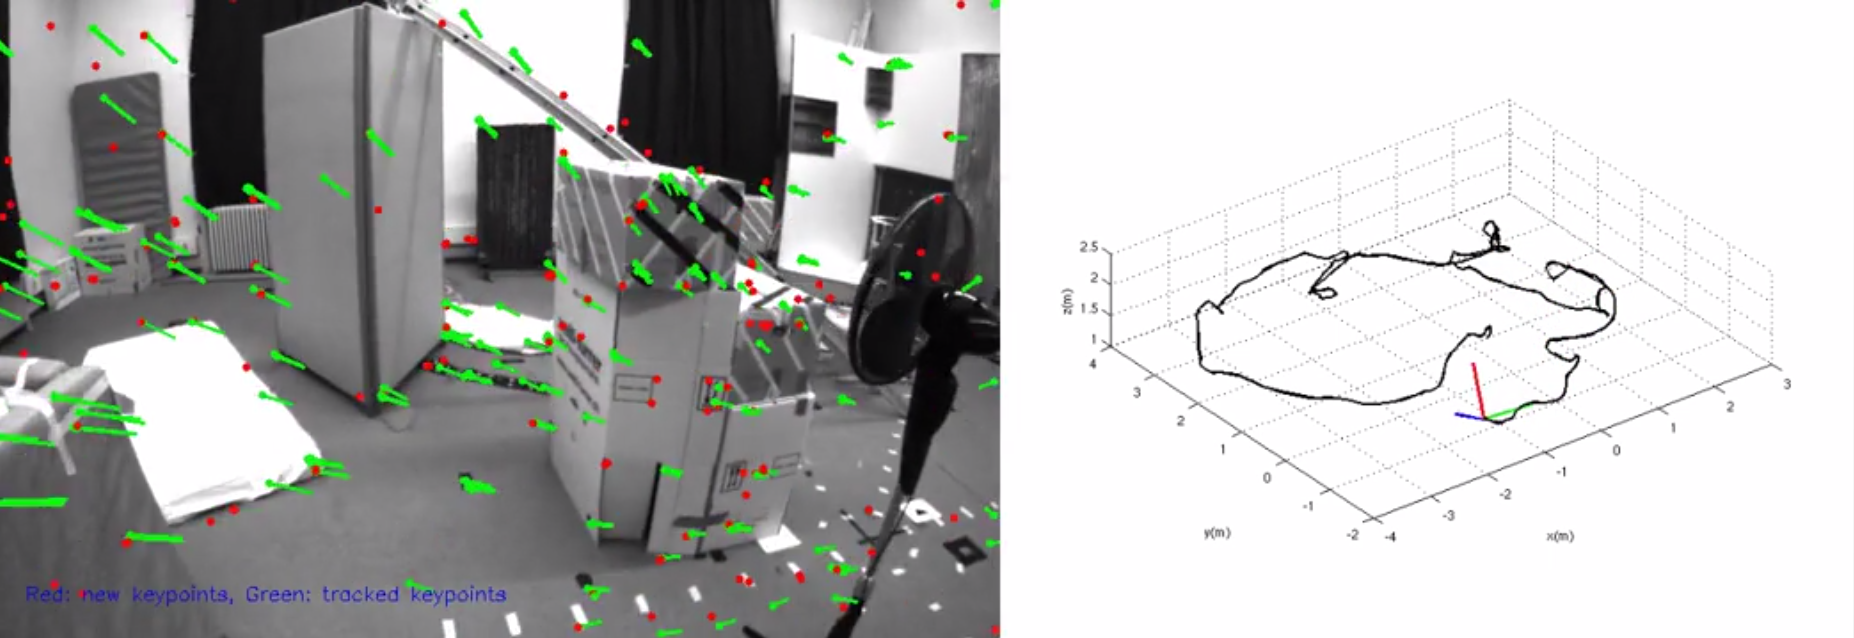
\includegraphics[width=0.7\columnwidth]{./figs/vins_paper_img.png}
\end{figure}

\item {\bf 3D Visual and Sound SLAM Mapping using a Handhold Integrated Visual Audio Sensor (Kinect and PS3 Eye)}\\
Sept, 2015 - Mar, 2017, at CAS, UTS.\\
Development of a SLAM package for Vision \& Sound joint mapping using C++ and Matlab (for simulation).\\
Visual features extraction, matching and visual place recognition using OpenCV and ORBSLAM frontend.\\
Sound sources state estimation by Extended Kalman Filter (EKF) with inverse depth parametrization and g2o (SLAM backend package) optimization.\\
Visual point cloud processing using PCL and Octo mapping.\\
Affiliated Video: \href{https://youtu.be/QyqY2eIX1wk}{https://youtu.be/QyqY2eIX1wk}.\\
\begin{figure}[H]
  \centering
  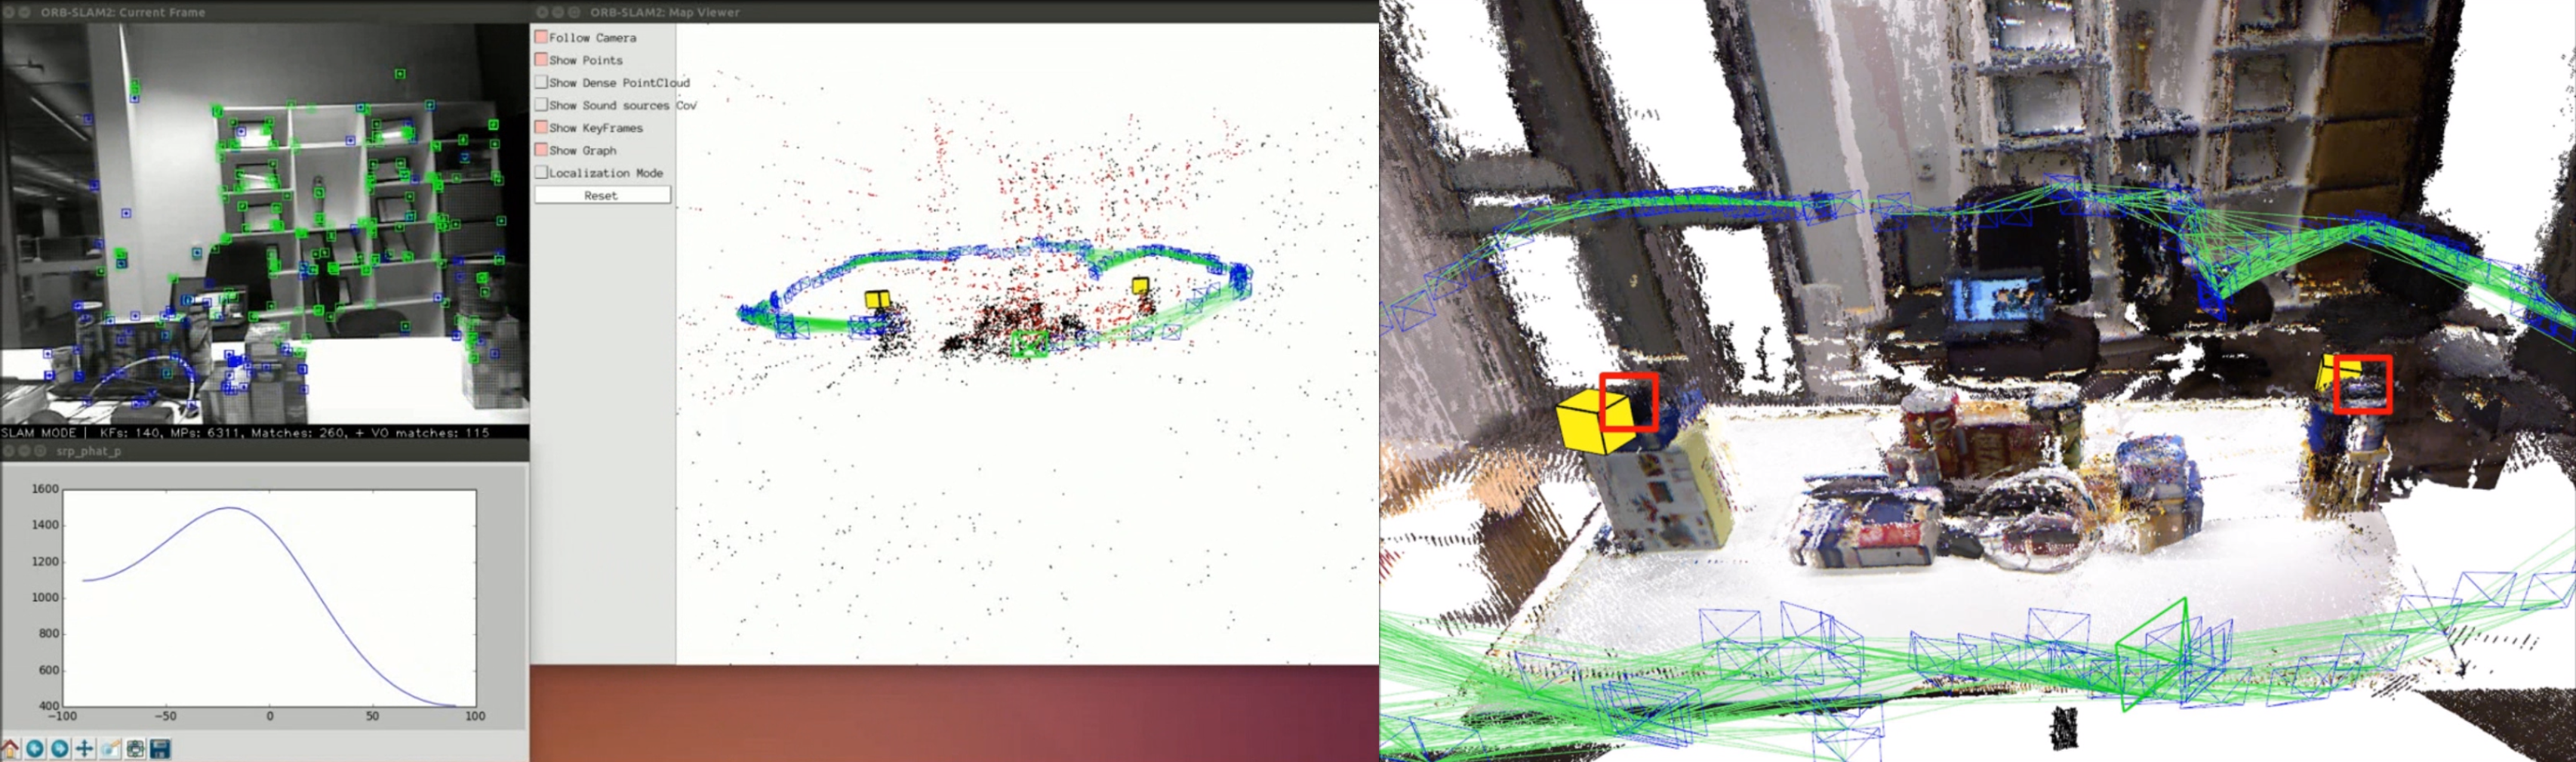
\includegraphics[width=0.7\columnwidth]{./figs/ssm_linear.png}
\end{figure}

\item {\bf 3D SLAM Mapping using Velodyne (3D laser scanner) and Kinect (RGBD camera) on Husky robot}\\
May, 2015 - Sept, 2015, at HRI-JP.\\
Interfacing Velodyne 3D laser scanner and Microsoft Kinect to PC.\\
Fine tuning SLAM packages LOAM and RGBDSLAM for 3D laser mapping using Velodyne and 3D visual mapping using Kinect (all using C++ and ROS).\\
(\textbf{confidential industry project})

\item {\bf Indoor sound mapping using a Turtlebot embedded with a laser scanner and microphone array}\\
May, 2015 - Sept, 2015, at HRI-JP.\\
Installation of external sensors and interfacing to PC.\\
Installation, debugging and tuning 2D SLAM packages using the Hokoyu laser range finder using ROS, Hector SLAM, C++.\\
Sound mapping by microphone array signal processing, ray tracing technique, sound sources clustering using ROS, C++ and Matlab.\\
Optimal path planning and navigation for exploration and optimal observation using ROS, Python and Matlab.\\
Setting up simulation using Gazebo and visualization using RViz.\\
\begin{figure}[H]
  \centering
  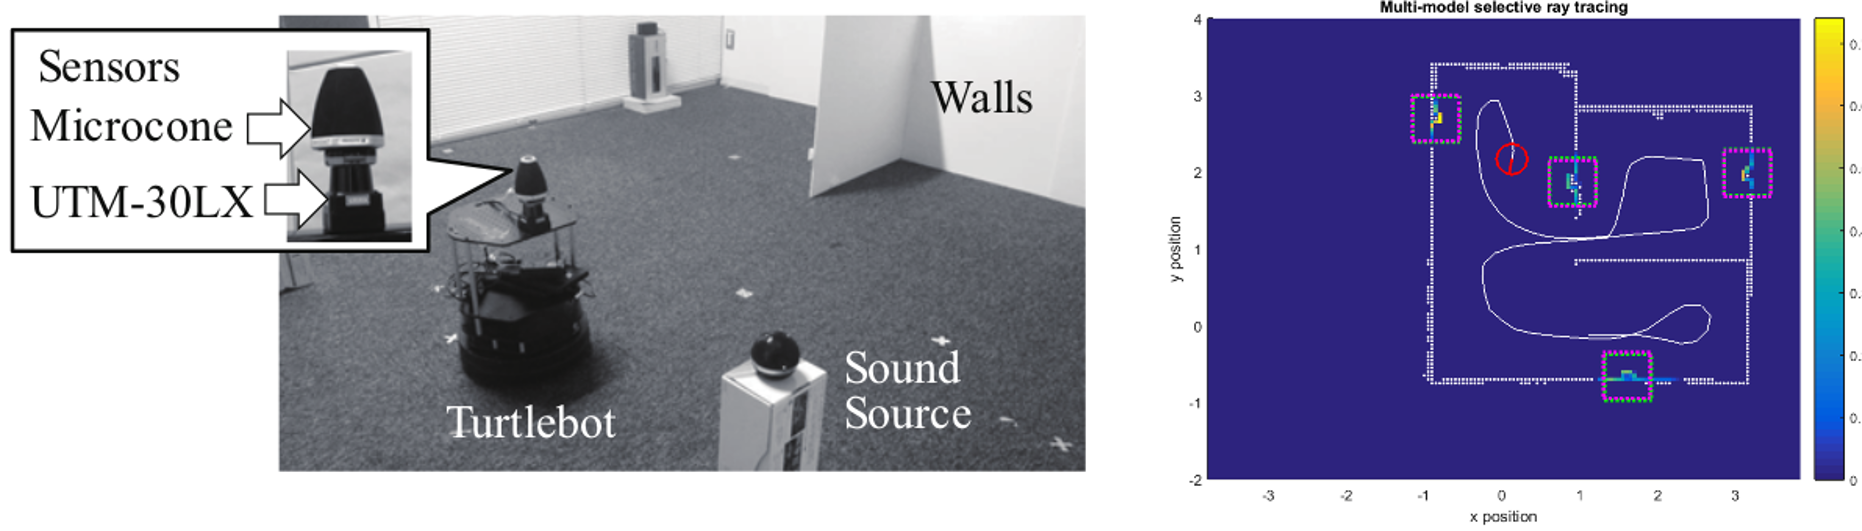
\includegraphics[width=0.8\columnwidth]{./figs/ssm_multi_model.png}
\end{figure}


\item {\bf Hardware and Software Design of GUTS Robot for Intelligent Tracking}\\
Oct, 2013 - Mar, 2017, at CAS UTS.\\
Design and installation of all electronics hardware related to sensors (sonar and IR array, RF transmitters, wheel encoders and cameras) and motor controller. \\
Designing some mechanical parts using Solidworks.\\
Programming embedded microcontrollers, establishing interfaces to PC and PID motor controller using C/C++.\\
Programming high level software: sensors signal processing, building probabilistic sensor model using machine learning technique, robot state estimation, robot navigation planning and visualization using ROS, C/C++, Python, GPy(Gaussian Process Python lib), Matlab Robotics Toolbox, Rviz, V-Rep(for simulation).\\
Affiliated Video: \href{https://youtu.be/hjLQfrdelcs}{https://youtu.be/hjLQfrdelcs}.\\
\begin{figure}[H]
  \centering
  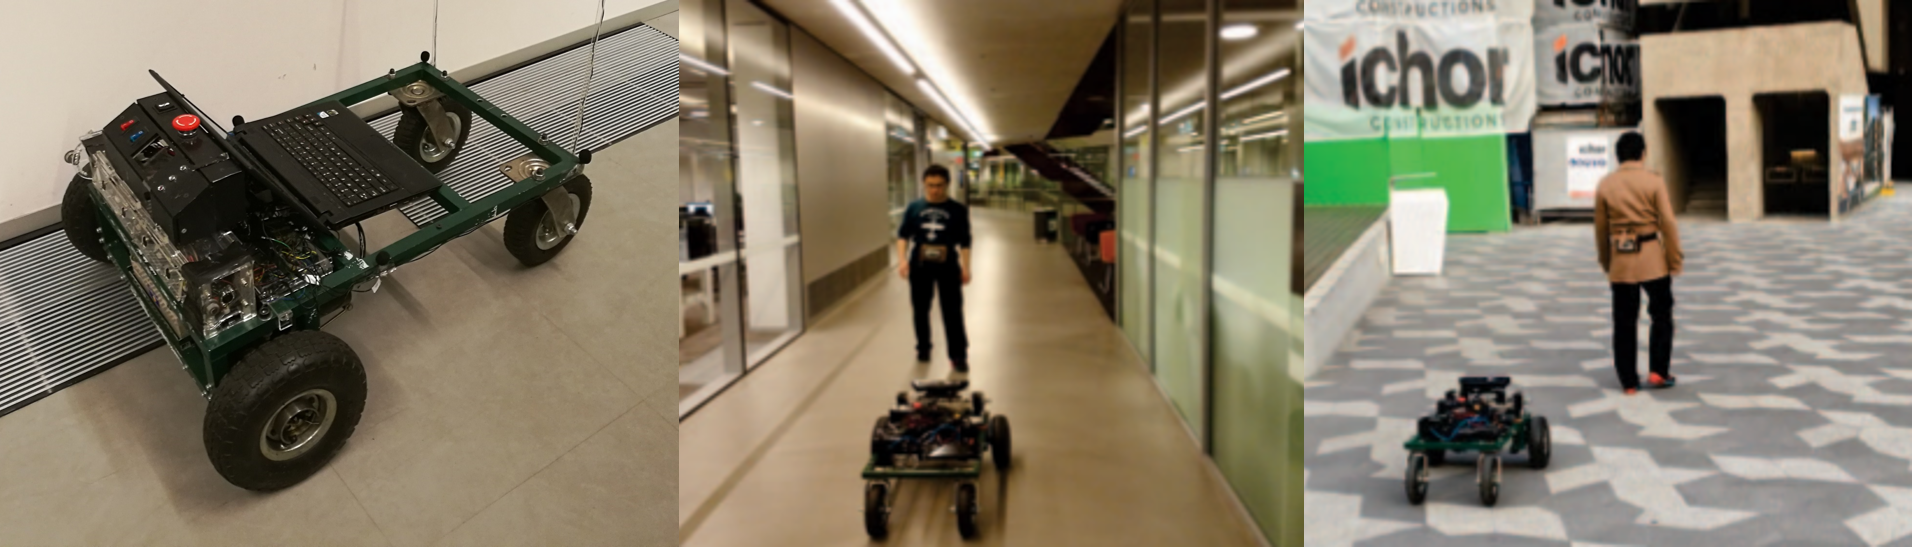
\includegraphics[width=0.99\columnwidth]{./figs/guts_tracking.png}
\end{figure}

\item {\bf  Designing Real-Time Robot Audition System for Speaker Identification and Tracking}\\
Apr, 2012 - Aug, 2012, at Keio University.\\
Features extraction and modelling using machine learning techniques (FMCC features and Gaussian Mixture Model)\\
Integrating, debugging and tuning multi-channel microphone array driver and other hardware interfaces (e.g. bluetooth interface) using C/C++.\\ 
Real-time microphone array signal processing for sound direction estimation and robust real-time tracking using ROS, C/C++.\\
Affiliated Video: \href{http://youtu.be/xMn4iih-akE}{http://youtu.be/xMn4iih-akE}.\\

%\item {\bf Erasmus Mundus Scholarship} for Master study as EMARO, funded by European Union, Approx. 10 scholarships available for applications from all over the world (outside Europe), 2010-2012.
%
%\item {\bf Academic Excellent Scholarship} by Zhejiang University, China.
\item {\bf Automatic Latin-letter recognition}\\
Oct, 2010 - Jan, 2011, at Warsaw University of Technology.\\
Image features extraction and Bayesian supervised learning using openCV, ROS and C++.\\

\end{itemize}



%%%%%%%%%%%%
\section{\sc Computer Skills} 
\begin{list2}
\item {\bf Programming}: Matlab, C/C++ and Python (good), Java and Unix/Linux kernel programming (acquired). \\

\item {\bf Robotics Libraries}: ROS, OpenCV, TensorFlow, Torch and V-REP (good), OpenGL, QT and PCL (acquired).\\

\item {\bf Hardware Design}: AutoCAD, Solidworks and ProE(good), Protel, Pspice and Multisim (acquired).\\

\item {\bf Simulation}: COMSOL Multi Physics (good), AnSys, Gambit and Fluid (acquired) \\
\end{list2}




%%%%%%%%%%%%
\section{\sc Language Skills} 
English: Professional (TOEFL ibt 108/120)\\
Chinese and Mongolian: Native\\
German and Japanese: Beginner

%%%%%%%%%%%%
\section{\sc Honors and Awards} 
\begin{itemize}


\item {\bf UTS IRS} %(International Research Scholarship) 
scholarship and {\bf UTS FEIT Faculty} scholarship for PhD study at UTS, 2013-2016.

%\vspace*{-2.5mm}
%NSF Vertical Integration of Research and Education in Statistics and
%Mathematical Sciences\\ (VIGRE) teaching fellowship.
%
\vspace*{-2.5mm}
\item {\bf Erasmus Mundus Scholarship} for Master study as EMARO, funded by European Union, Approx. 10 scholarships available for applications from all over the world (outside Europe), 2010-2012.

\vspace*{-2.5mm}
\item {\bf Academic Excellent Scholarship} by Zhejiang University, China.

\vspace*{-2.5mm}
\item {\bf Tuition Wave Scholarship} 4 times in Academic year 2006-2010 by Zhejiang University, China.

\vspace*{-2.5mm}
\item {\bf National Stipend} 4 times in Academic year 2006-2010, funded by Chinese Ministry of Education

\vspace*{-2.5mm}
\item 1st Prize in {\bf Mechatronic System Design Competition} in Zhejiang Uni. Oct, 2009-Feb, 2010

\vspace*{-2.5mm}
\item 1st Prize out of 1620 teams from 159 universities/colleges/institutes in {\bf National Energy Saving and Emission Reduction Competition} Feb, 2009-Sep, 2009


\end{itemize}


%%%%%%%%%%%%
\section{\sc Publications}
%Paciorek, C.J., J.S. Risbey, V. Ventura, and R.D.Rosen. 2002. Multiple indices of Northern Hemisphere Cyclone
%Activity, Winters 1949-1999. Journal of Climate 15:1573-1590.
%
%Paciorek, C.J., R. Condit, S.P. Hubbell, and R.B. Foster.  2000.
%The demographics of resprouting in tree and shrub species of a moist
%tropical forest.  Journal of Ecology 88:765-777.
%
%Paciorek, C.J., B.R. Moyer, R.A. Levin, and S.L. Halpern.  1995.
%Pollen consumption by hummingbird flower mite {\it Proctolaelaps
%  kirmsei} and possible fitness effects on {\it Hamelia patens}.
%Biotropica 27:258-262.  (author order determined by lot)
\textbf{Journal Publications}

\begin{enumerate}

\item \textbf{Daobilige Su}, Yongliang Qiao, He Kong, and Salah Sukkarieh, ``Real Time Detection of Inter-Row Ryegrass in Wheat Farm using Deep Learning'', \textbf{under review} in \textit{European Journal of Agronomy}, 2019. (2019 IF \textbf{3.384})

\item He Kong, Mao Shan, \textbf{Daobilige Su}, Yongliang Qiao, Abdullah Al-Azzawi, and Salah Sukkarieh, ``Filtering for Systems subject to Unknown Inputs without Apriori Initial Information'', \textbf{under review} in \textit{Automatica}, 2019. (2019 IF  \textbf{6.355})

\item \textbf{Daobilige Su}, He Kong, and Salah Sukkarieh, ``Data Augmentation for Deep Learning based Semantic Segmentation and Crop-Weed Classification in Agricultural Robotics'', \textbf{under review} in \textit{Biosystems Engineering}, 2019. (2019 IF  \textbf{2.983})

\item Jasper Brown, \textbf{Daobilige Su}, He Kong, Salah Sukkarieh, and Eric Kerrigan. ``Improved Noise Covariance Estimation in Visual Servoing Using an Autocovariance Least-squares Approach'', \textbf{invited paper} to \textit{Mechatronics}, 2019. (2019 IF \textbf{2.978})

\item {\bf Daobilige Su}, Teresa Vidal Calleja and Jaime Valls Miro, ``Simultaneous asynchronous microphone array calibration and sound source localisation'', {\it Autonomous Robots}, pp. 1-22, 2019. (2019 IF \textbf{3.634})

% Yongliang Qiao, Salah Sukkarieh and Daobilige Su, Animal Sound Detection and Clustering using Manifold Regularized Deep Learning
%\item Yongliang Qiao, Salah Sukkarieh, {\bf Daobilige Su}, ``Animal Sound Detection and Clustering using Manifold Regularized Deep Learning'', \textbf{accepted} in {\it Sensors}, 2018. (2018 \textbf{IF 2.475})

% Su, Daobilige, Asher Bender, and Salah Sukkarieh. "Improved Cross-Ratio Invariant-Based Intrinsic Calibration of A Hyperspectral Line-Scan Camera." Sensors 18, no. 6 (2018): 1885.
\item {\bf Daobilige Su}, Asher Bender and Salah Sukkarieh, ``Improved Cross-Ratio Invariant-Based Intrinsic Calibration of A Hyperspectral Line-Scan Camera'', in {\it Sensors}, vol. 18 no. 6, pp. 1885, 2018. (2019 \textbf{IF 3.031})

% Wang, Mengmeng, Yong Liu, Daobilige Su, Yufang Liao, Lei Shi, and Jinhong Xu. "Accurate and Real-time 3D Tracking for the Following Robots by Fusing Vision and Ultra-sonar Information." IEEE/ASME Transactions on Mechatronics (2018).
\item Mengmeng Wang, Yong Liu, {\bf Daobilige Su}, Yufang Liao, Lei Shi, Jinhong Xu and Jaime Valls Miro, ``Accurate and Real-time 3D Tracking for the Following Robots by Fusing Vision and Ultrasonar Information'', in {\it IEEE/ASME Transactions on Mechatronics}, vol. 23 no. 3, pp. 997-1006, 2018. (2018 \textbf{IF 3.936})
\end{enumerate}

\textbf{Conference Publications}
\begin{enumerate}

% Brown, Jasper, Daobilige Su, He Kong, Salah Sukkarieh, and Eric Kerrigan. "Improved Noise Covariance Estimation in Visual Servoing Using an Autocovariance Least-squares Approach."
%The 12th IFAC Conference on Control Applications in Marine Systems, Robotics, and Vehicles (CAMS 2019) and the first workshop on Robot Control (WROCO 2019)
\item Jasper Brown, \textbf{Daobilige Su}, He Kong, Salah Sukkarieh, and Eric Kerrigan. ``Improved Noise Covariance Estimation in Visual Servoing Using an Autocovariance Least-squares Approach'', in \textit{Joint 12th IFAC Conference on Control Applications in Marine Systems, Robotics, and Vehicles (CAMS 2019) and the first workshop on Robot Control (WROCO 2019)}, 2019.

% Wang, Min, Holger Voos, and Daobilige Su. "Robust Online Obstacle Detection and Tracking for Collision-Free Navigation of Multirotor UAVs in Complex Environments." In 2018 15th International Conference on Control, Automation, Robotics and Vision (ICARCV), pp. 1228-1234. IEEE, 2018.
\item Min Wang, Holger Voos and {\bf Daobilige Su}, ``Robust Online Obstacle Detection and Tracking for Collision-free Navigation of Multirotor UAVs in Complex Environments'', in {\it 2018 15th International Conference on Control Automation Robotics \& Vision (ICARCV 2018)}, pp. 1228-1234, 2018.

% KANZHI WU, Teng Zhang*, Daobilige Su, Shoudong Huang, Gamini Dissanayake
% An Invariant-EKF VINS Algorithm for Improving Consistency
% Wu, Kanzhi, Teng Zhang, Daobilige Su, Shoudong Huang, and Gamini Dissanayake. "An invariant-EKF VINS algorithm for improving consistency." In Intelligent Robots and Systems (IROS), 2017 IEEE/RSJ International Conference on, pp. 1578-1585. IEEE, 2017.
\item Kanzhi Wu*, Teng Zhang*, {\bf Daobilige Su}, Shoudong Huang, Gamini Dissanayake, ``An Invariant-EKF VINS Algorithm for Improving Consistency'', in {\it 2017 IEEE/RSJ International Conference on Intelligent Robots and Systems (\textbf{IROS 2017})}, pp. 1578-1585, 2017.
(* indicates equal contribution)

% Su, Daobilige, Teresa Vidal-Calleja, and Jaime Valls Miro. "Towards real-time 3D sound sources mapping with linear microphone arrays." In Robotics and Automation (ICRA), 2017 IEEE International Conference on, pp. 1662-1668. IEEE, 2017.
\item {\bf Daobilige Su}, Teresa Vidal Calleja and Jaime Valls Miro, ``Towards Real-Time 3D Sound Sources Mapping with Linear Microphone Arrays'', in {\it 2017 IEEE International Conference on Robotics and Automation (\textbf{ICRA 2017})}, pp. 1662-1668, 2017.
%2017. 
(Affiliated Video: \\ \href{https://youtu.be/Ry_i3kmvlHM}{{https://youtu.be/Ry\_i3kmvlHM}}, Open source code: \\ \href{https://github.com/daobilige-su/SSM_LinearArray}{{https://github.com/daobilige-su/SSM\_LinearArray}})

% Wang, Mengmeng, Daobilige Su, Lei Shi, Yong Liu, and Jaime Valls Miro. "Real-time 3D human tracking for mobile robots with multisensors." In Robotics and Automation (ICRA), 2017 IEEE International Conference on, pp. 5081-5087. IEEE, 2017.
\item Mengmeng Wang, {\bf Daobilige Su}, Lei Shi, Yong Liu and Jaime Valls Miro, ``Real-time 3D Human Tracking for Mobile Robots with Multisensors'', in {\it 2017 IEEE International Conference on Robotics and Automation (\textbf{ICRA 2017})}, pp. 5081-5087, 2017.

\item {\bf Daobilige Su}, Teresa Vidal Calleja and Jaime Valls Miro, ``Split Conditional Independent Mapping for Sound Source Localisation with Inverse-Depth Parametrisation'', in {\it 2016 IEEE/RSJ International Conference on Intelligent Robots and Systems (\textbf{IROS 2016})}, pp. 2000-2006, 2016. (Affiliated Video: \href{https://youtu.be/QyqY2eIX1wk}{{https://youtu.be/QyqY2eIX1wk}})

\item {\bf Daobilige Su}, Keisuke Nakamura, Kazuhiro Nakadai and Jaime Valls Miro, ``Robust Sound Source Mapping using Three-layered Selective Audio Rays for Mobile Robots'', in {\it 2016 IEEE/RSJ International Conference on Intelligent Robots and Systems (\textbf{IROS 2016})}, pp. 2771-2777, 2016.

\item {\bf Daobilige Su}, Teresa Vidal Calleja and Jaime Valls Miro, ``Simultaneous asynchronous microphone array calibration and sound source localisation'', in {\it 2015 IEEE/RSJ International Conference on Intelligent Robots and Systems (\textbf{IROS 2015})}, pp. 5561-5567, 2015.

\item {\bf Daobilige Su}, Jaime Valls Miro and Teresa Vidal Calleja, ``Graph-SLAM Based Calibration of an Embedded Asynchronous Microphone Array for Outdoor Robotic Target Tracking'', in {\it Assistive Robotics: Proceedings of the 18th International Conference on CLAWAR 2015}, pp. 641-648, 2015. ({\bf Best Paper Award Finalist}).

\item {\bf Daobilige Su}, Jaime Valls Miro and Teresa Vidal Calleja, ``Real-time sound source localisation for target tracking applications using an asynchronous microphone array'', in {\it 2015 IEEE 10th Conference on Industrial Electronics and Applications (ICIEA 2015)}, pp. 1261-1266, 2015.

\item {\bf Daobilige Su}, Jaime Valls Miro and Teresa Vidal Calleja, ``Modelling in-pipe acoustic signal propagation for condition assessment of multi-layer water pipelines'', in {\it 2015 IEEE 10th Conference on Industrial Electronics and Applications (ICIEA 2015)}, pp. 545-550, 2015. ({\bf Best Paper Award Finalist}).

\item {\bf Daobilige Su}, Nalika Ulapane and Buddhi Wijerathna, ``An acoustic sensor based novel method for 2D localization of a robot in a structured environment'', in {\it 2015 IEEE 10th Conference on Industrial Electronics and Applications (ICIEA 2015)}, pp. 2024-2029, 2015.

\item {\bf Daobilige Su} and Jaime Valls Miro. ``An ultrasonic/RF GP-based sensor model robotic solution for indoors/outdoors person tracking'', in {\it 2014 13th International Conference on Control Automation Robotics \& Vision (ICARCV 2014)}, pp. 1662-1667, 2014.

\item Teresa Vidal Calleja, {\bf Daobilige Su}, Freek De Bruijn and Jaime Valls Miro, ``Learning spatial correlations for Bayesian fusion in pipe thickness mapping'', in {\it 2014 IEEE International Conference on Robotics and Automation (\textbf{ICRA 2014})}, pp. 683-690, 2014.

\item Jaime Valls Miro, Jeya Rajalingam, Teresa Vidal Calleja, Freek de Bruijn, Roger Wood, Dammika Vitanage, Nalika Ulapane, Buddhi Wijerathna and {\bf Daobilige Su}, ``A live test-bed for the advancement of condition assessment and failure prediction research on critical pipes'', in {\it Proceedings of the Leading-Edge Strategic Asset Management Conference (LESAM13)}. 2013.

\item {\bf Daobilige Su}, Masashi Sekikawa, Kazuo Nakazawa and Nozomu Hamada, ``Novel scheme of real-time direction finding and tracking of multiple speakers by robot-embedded microphone array'', in {\it the 1st International Conference on Robot Intelligence Technology and Applications (RITA 2012)}, 2012.

\end{enumerate}




%\vspace{-.3cm}
%{\em Graduate Student} \hfill {\bf August, 1998 - present}\\
%Includes current Ph.D.~research, Ph.D.~and Masters level coursework and
%research/consulting projects.
%
%%\vspace{-.1cm}
%{\em Instructor} \hfill {\bf May - June, 2002}\\
%Co-taught graduate level course for the Master of Science in
%Computational Finance program.  Shared responsibility for lectures, exams,
%homework assignments, and  grades.  
%\vspace*{.05in}  
%\begin{list2}
%\item 46-731 Probability and Statistics, Summer 2002.
%\end{list2}


%%\vspace{-.1cm}
%{\em NSF VIGRE Teaching Fellow} \hfill {\bf January - May, 2001}\\
%Head teaching assistant.   
%Duties included  shared administrative responsibilities with faculty
%instructor, fielding of all student inquiries, and oversight of
%graduate student teaching assistants and graders.
%\vspace*{.05in}  
%\begin{list2}
%\item 36-217 Probability Theory and Random Processes, Spring 2001.
%\end{list2}
%
%%\vspace{-.1cm}
%{\em Teaching Assistant} \hfill {\bf August, 2001  - present}\\
%Duties at various times have included 
%office hours and leading weekly computer lab exercises.


   


%%%%%%%%%%%%
%\section{\sc Papers in preparation}
%
%Ventura, V., C.J. Paciorek, and J.S. Risbey.  Controlling the proportion of falsely-rejected hypotheses when conducting multiple tests with geophysical data.
%
%Ickes, K., C.J. Paciorek, and S. Thomas.  Effects of wild pigs on
%forest demographic processes in Malaysia.
%
%

%%%%%%%%%%%%
%\section{\sc Conference Presentations}
%Paciorek, C.J., J.S. Risbey, V. Ventura, and R.D.Rosen.  2001.  Changes in Northern Hemisphere winter storm activity (1949-1999) based
%on a comparison of cyclone indices.  8th International Meeting on
%Statistical Climatology, Luneberg, Germany, March, 2001.
%
%Paciorek, C.J. and R. Rosenfeld.  2000.  Minimum classification error
%training in exponential language models.  2000 Spring Transcription
%Workshop, College Park, Maryland.
%\vspace*{-.25in}  
%\begin{verbatim}http://www.nist.gov/speech/publications/tw00/html/abstract.htm#cp1-50\end{verbatim}
%
%
%

%%%%%%%%%%%%
%\section{\sc Professional Experience}
%{\bf Bureau of Transportation Statistics, U.S. Department of
%  Transportation}, Washington, District of Columbia USA
%
%\vspace{-.3cm}
%{\em Summer researcher} \hfill {\bf May, 2000 - August, 2000}\\
%Carried out several consulting projects, including modelling of
%injuries to cadavers in crash test experiments, analysis of airline
%delay data, and advice on analysis of airline economics data.
%
%{\bf Abt Associates}, Bethesda, Maryland USA
%
%\vspace{-.3cm}
%{\em Associate Programmer Analyst and Research Assistant} \hfill {\bf
%  October, 1994 - August, 1996}\\
%Researcher and computer model developer for U.S. EPA Regulatory Impact
%Analysis of Section 403 Lead Paint Hazard Rule.  Other projects
%included database analysis, literature reviews, and cost-benefit analysis.







\end{resume}
\end{document}




